\section{Problem 2}
\label{part2}
\subsection*{Question}
\begingroup
\begin{verbatim}
We know the group split in two different groups.  Suppose the
disagreements in the group were more nuanced -- what would the clubs
look like if they split into groups of 3, 4, and 5?
\end{verbatim}

\begin{enumerate}
\item I used the same R script shown in Listing\ref{lst:q1codeR} to produce Figure\ref{fig:club-3-split}, \ref{fig:club-4-split} and \ref{fig:club-5-split}. The value of the \emph{threshold} is changed to 3, 4 or 5 as required to create the split. Even after spliting the karate club into 3, 4 or 5 groups Mr.Hi and John A hold the biggest groups. 
\end{enumerate}

\begin{figure}[h]
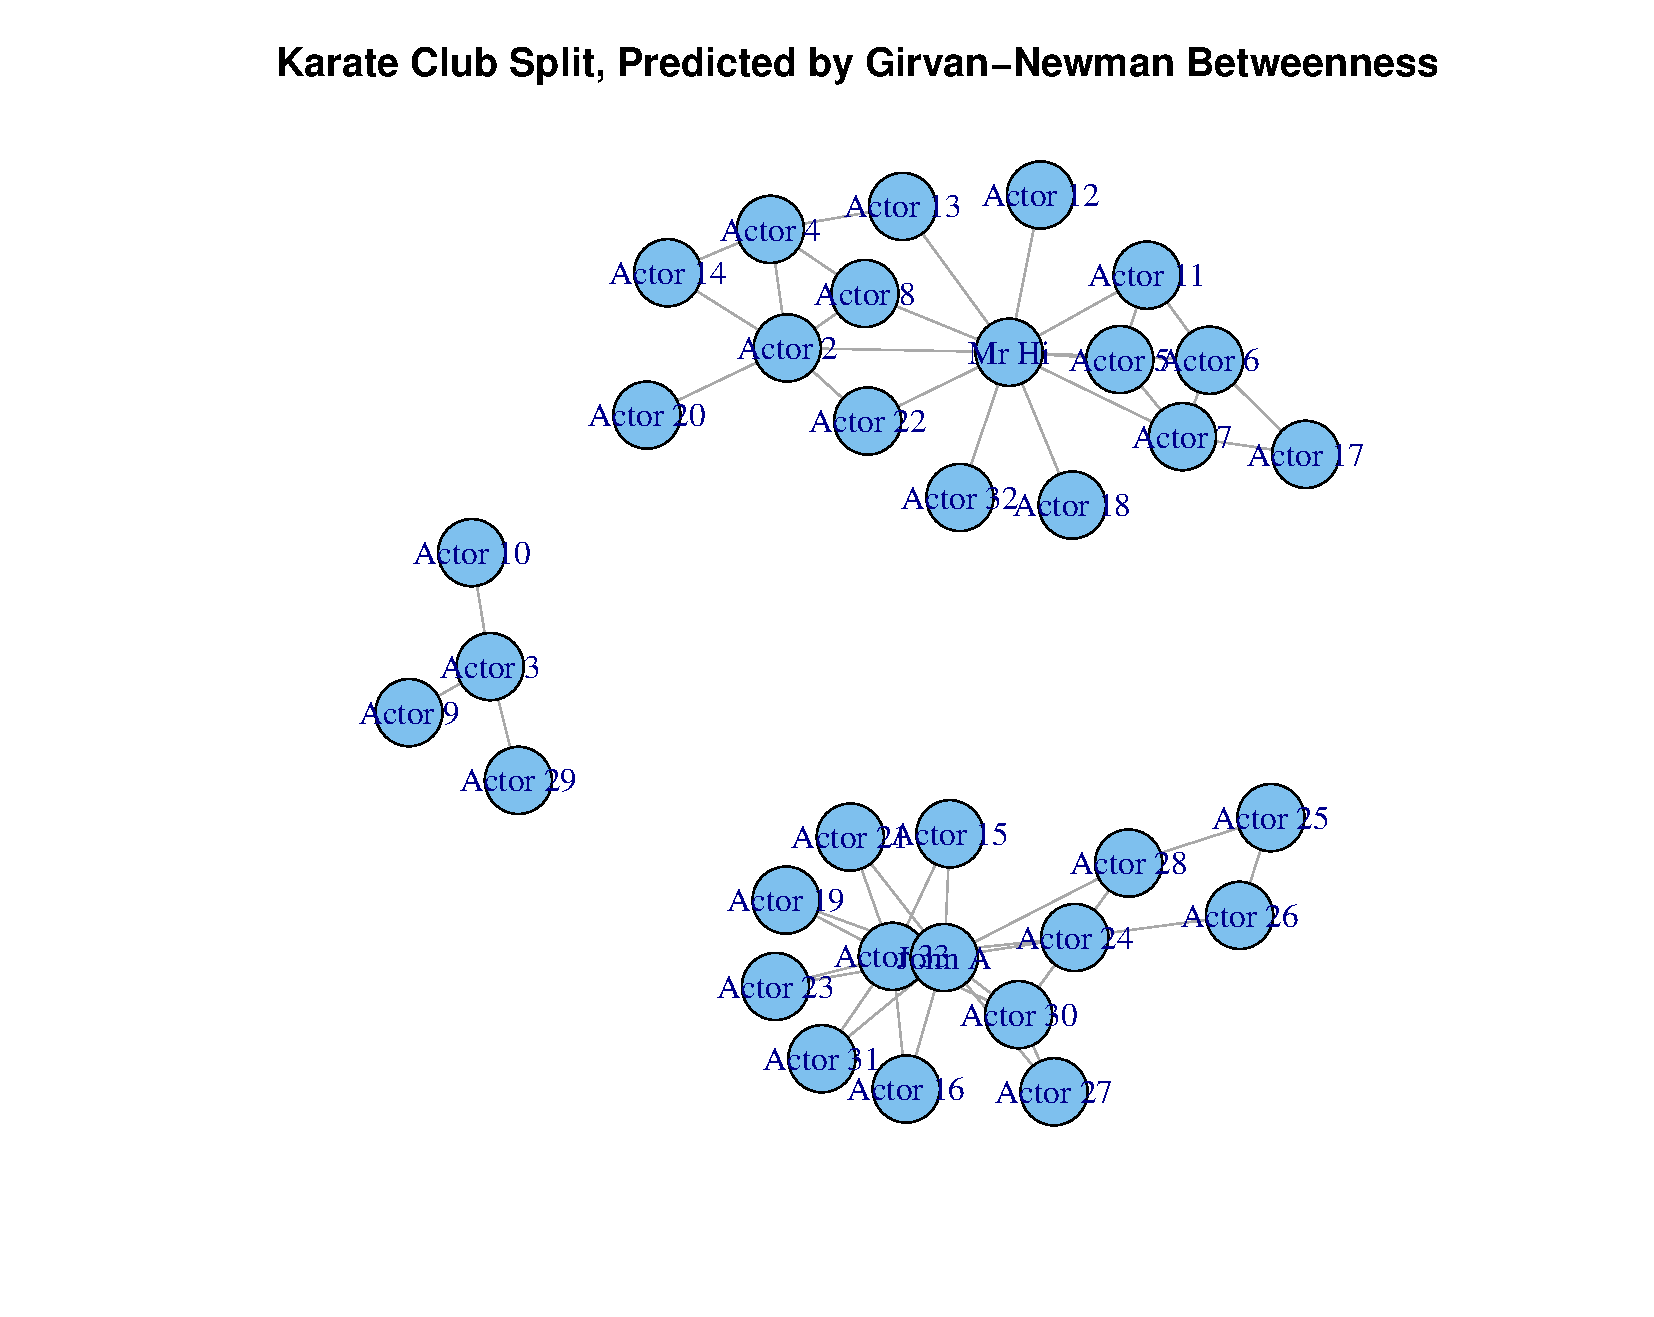
\includegraphics[scale=0.6]{R/group-of-3.pdf}
\caption{Karate Club Graph Split Into 3 Groups Predicted by Girvan \& Newman Betweenness Clustering}
\label{fig:club-3-split}
\end{figure}

\begin{figure}[h]
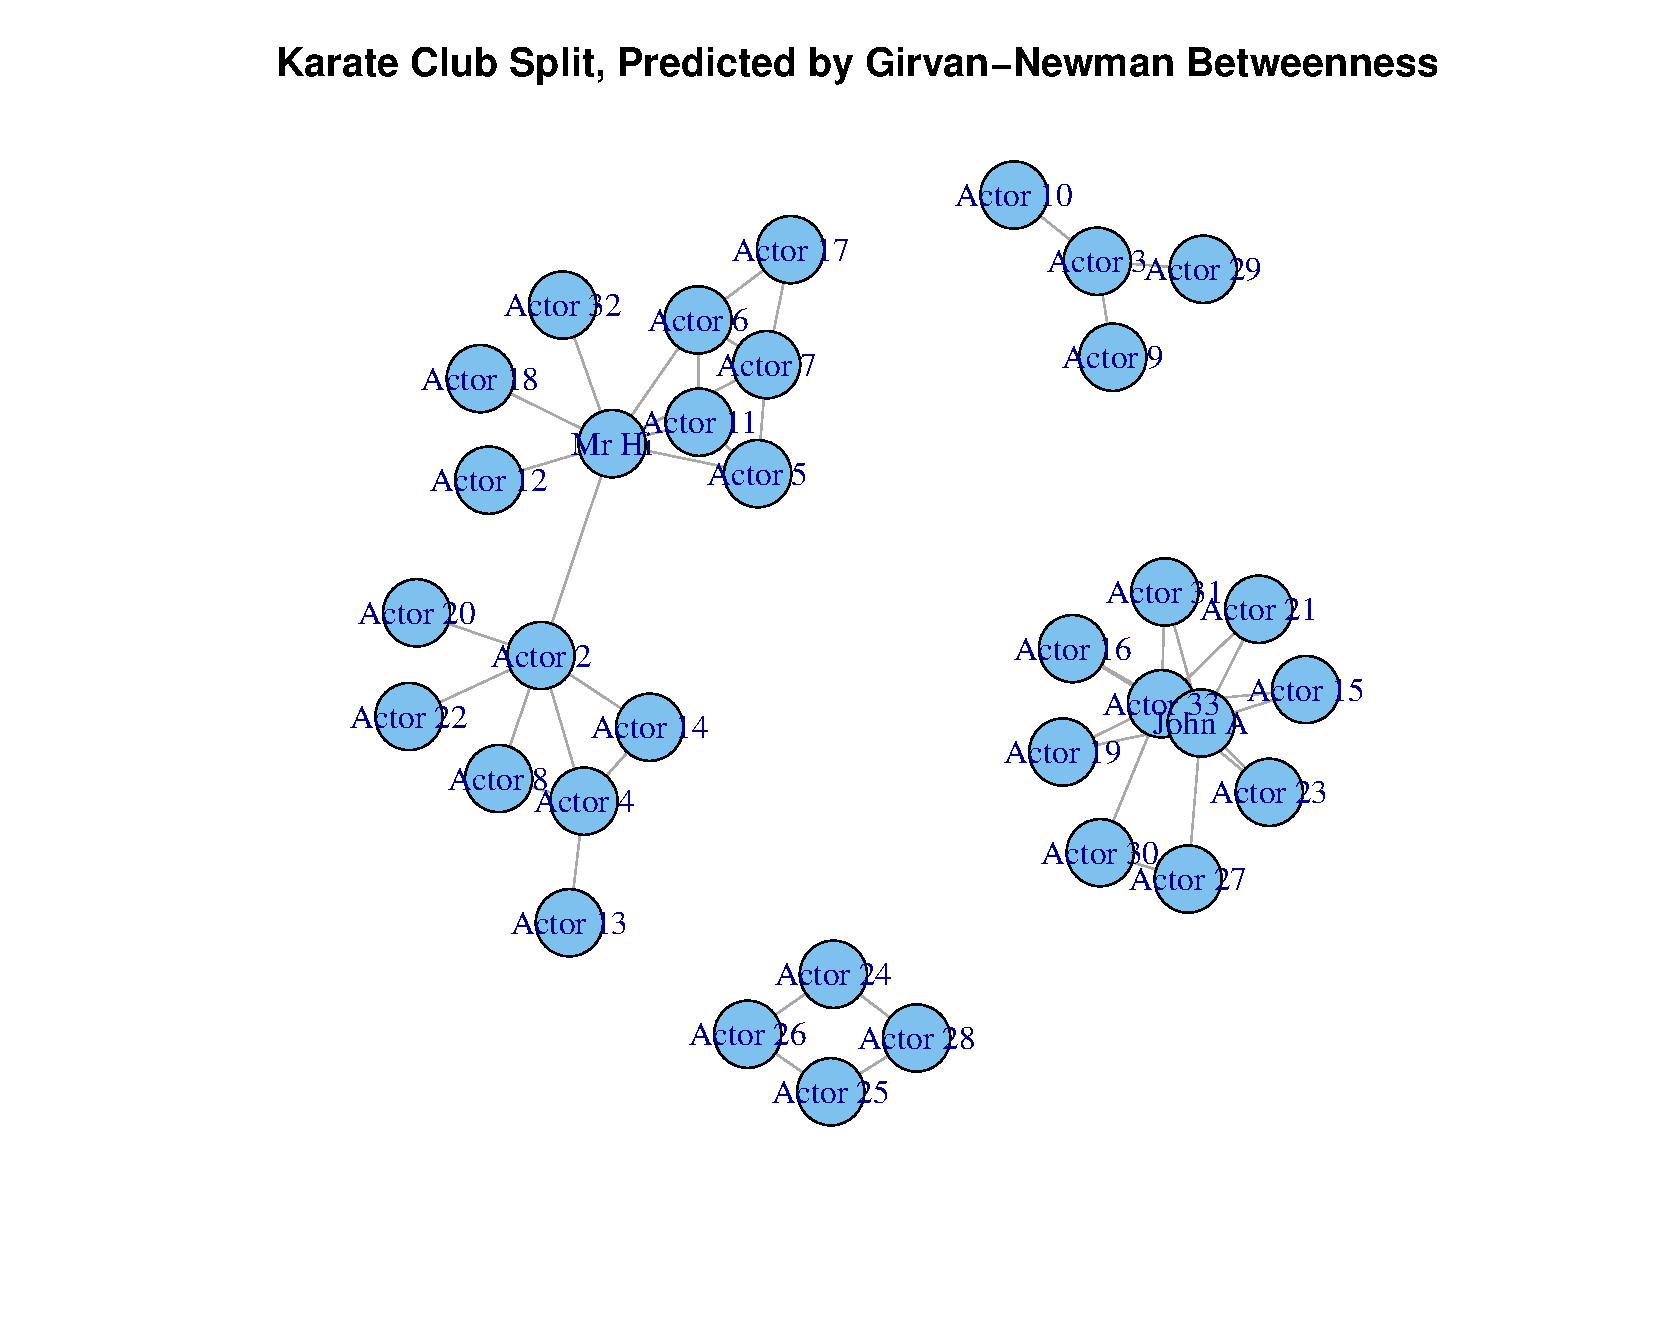
\includegraphics[scale=0.6]{R/group-of-4.pdf}
\caption{Karate Club Graph Split Into 4 Groups Predicted by Girvan \& Newman Betweenness Clustering}
\label{fig:club-4-split}
\end{figure}

\begin{figure}[h]
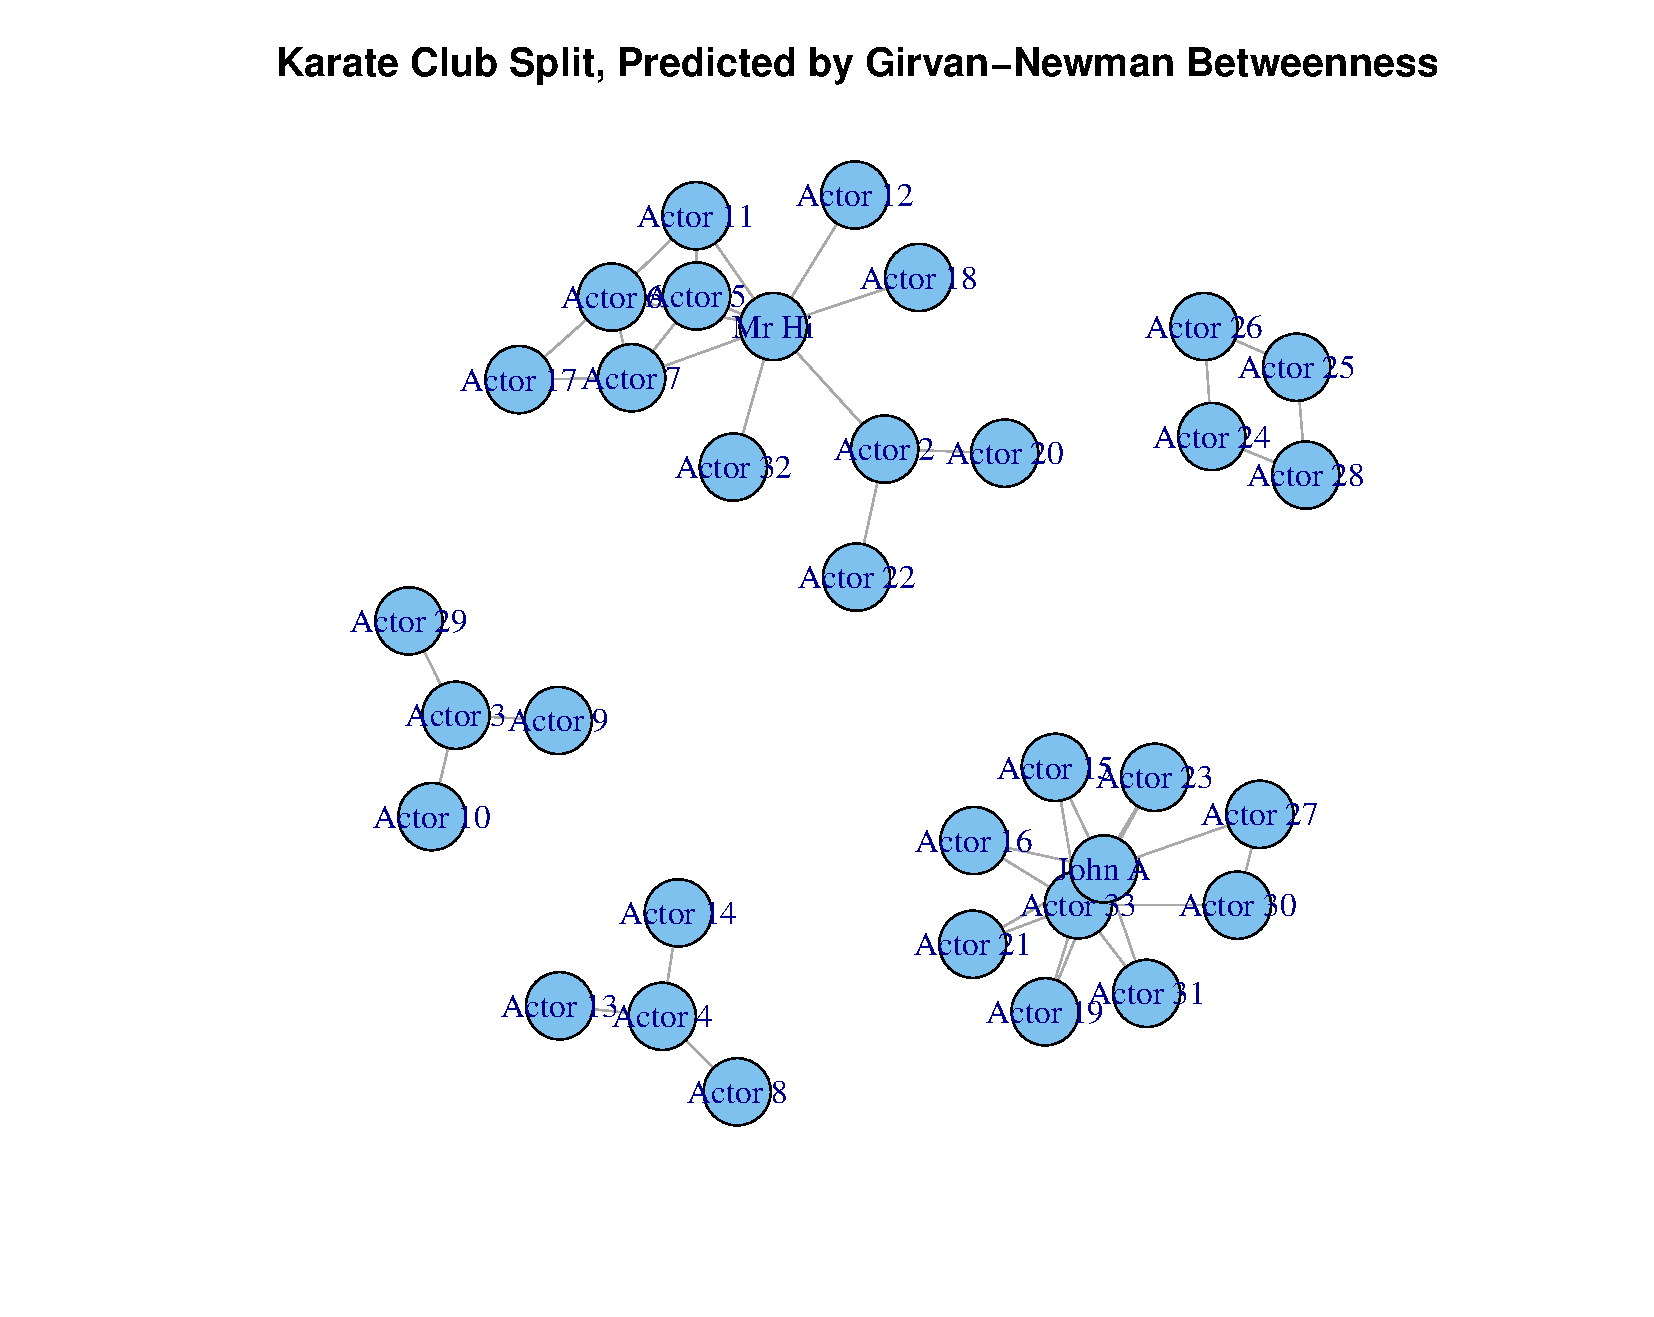
\includegraphics[scale=0.6]{R/group-of-5.pdf}
\caption{Karate Club Graph Split Into 5 Groups Predicted by Girvan \& Newman Betweenness Clustering}
\label{fig:club-5-split}
\end{figure}
